\documentclass{article}
\usepackage{tikz}
\begin{document}
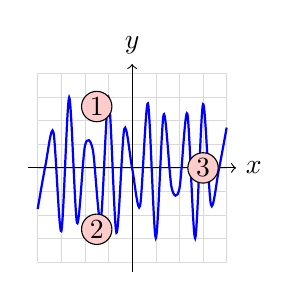
\begin{tikzpicture}[scale=0.6]
\draw[step=0.5,gray!30,very thin] (-2,-2) grid (2,2);
\draw[->] (-2.2,0) -- (2.2,0) node[right] {$x$};
\draw[->] (0,-2.2) -- (0,2.2) node[above] {$y$};
\draw[domain=-2:2,smooth,variable=\x,blue,thick] plot ({\x},{sin(\x*60 r)*1.5});
\foreach \a in {1,...,3} \node[circle,draw,fill=red!20,inner sep=1pt] at ({360/3*\a}:1.5) {\a};
\end{tikzpicture}
\par\medskip
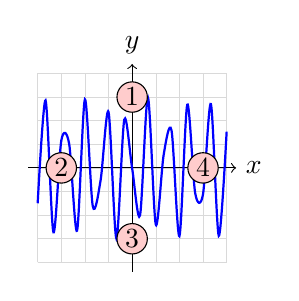
\begin{tikzpicture}[scale=0.6]
\draw[step=0.5,gray!30,very thin] (-2,-2) grid (2,2);
\draw[->] (-2.2,0) -- (2.2,0) node[right] {$x$};
\draw[->] (0,-2.2) -- (0,2.2) node[above] {$y$};
\draw[domain=-2:2,smooth,variable=\x,blue,thick] plot ({\x},{sin(\x*61 r)*1.5});
\foreach \a in {1,...,4} \node[circle,draw,fill=red!20,inner sep=1pt] at ({360/4*\a}:1.5) {\a};
\end{tikzpicture}
\par\medskip
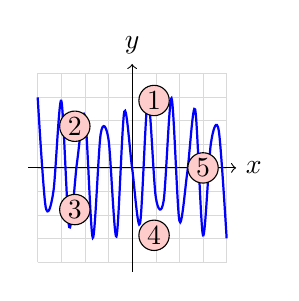
\begin{tikzpicture}[scale=0.6]
\draw[step=0.5,gray!30,very thin] (-2,-2) grid (2,2);
\draw[->] (-2.2,0) -- (2.2,0) node[right] {$x$};
\draw[->] (0,-2.2) -- (0,2.2) node[above] {$y$};
\draw[domain=-2:2,smooth,variable=\x,blue,thick] plot ({\x},{sin(\x*62 r)*1.5});
\foreach \a in {1,...,5} \node[circle,draw,fill=red!20,inner sep=1pt] at ({360/5*\a}:1.5) {\a};
\end{tikzpicture}
\par\medskip
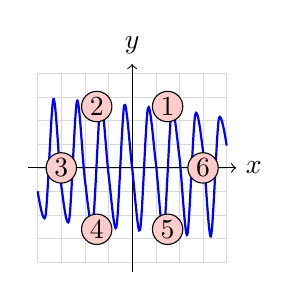
\begin{tikzpicture}[scale=0.6]
\draw[step=0.5,gray!30,very thin] (-2,-2) grid (2,2);
\draw[->] (-2.2,0) -- (2.2,0) node[right] {$x$};
\draw[->] (0,-2.2) -- (0,2.2) node[above] {$y$};
\draw[domain=-2:2,smooth,variable=\x,blue,thick] plot ({\x},{sin(\x*63 r)*1.5});
\foreach \a in {1,...,6} \node[circle,draw,fill=red!20,inner sep=1pt] at ({360/6*\a}:1.5) {\a};
\end{tikzpicture}
\par\medskip
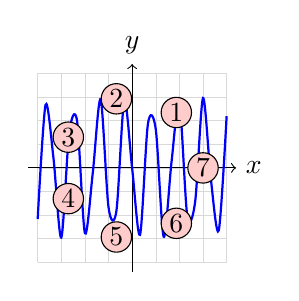
\begin{tikzpicture}[scale=0.6]
\draw[step=0.5,gray!30,very thin] (-2,-2) grid (2,2);
\draw[->] (-2.2,0) -- (2.2,0) node[right] {$x$};
\draw[->] (0,-2.2) -- (0,2.2) node[above] {$y$};
\draw[domain=-2:2,smooth,variable=\x,blue,thick] plot ({\x},{sin(\x*64 r)*1.5});
\foreach \a in {1,...,7} \node[circle,draw,fill=red!20,inner sep=1pt] at ({360/7*\a}:1.5) {\a};
\end{tikzpicture}
\par\medskip
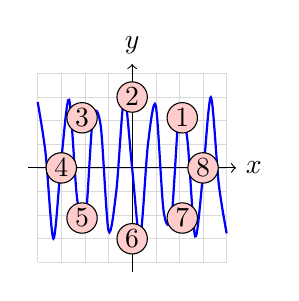
\begin{tikzpicture}[scale=0.6]
\draw[step=0.5,gray!30,very thin] (-2,-2) grid (2,2);
\draw[->] (-2.2,0) -- (2.2,0) node[right] {$x$};
\draw[->] (0,-2.2) -- (0,2.2) node[above] {$y$};
\draw[domain=-2:2,smooth,variable=\x,blue,thick] plot ({\x},{sin(\x*65 r)*1.5});
\foreach \a in {1,...,8} \node[circle,draw,fill=red!20,inner sep=1pt] at ({360/8*\a}:1.5) {\a};
\end{tikzpicture}
\par\medskip
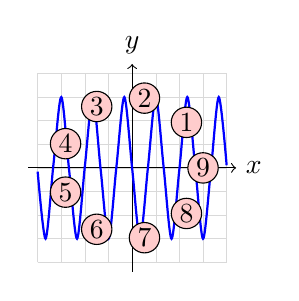
\begin{tikzpicture}[scale=0.6]
\draw[step=0.5,gray!30,very thin] (-2,-2) grid (2,2);
\draw[->] (-2.2,0) -- (2.2,0) node[right] {$x$};
\draw[->] (0,-2.2) -- (0,2.2) node[above] {$y$};
\draw[domain=-2:2,smooth,variable=\x,blue,thick] plot ({\x},{sin(\x*66 r)*1.5});
\foreach \a in {1,...,9} \node[circle,draw,fill=red!20,inner sep=1pt] at ({360/9*\a}:1.5) {\a};
\end{tikzpicture}
\par\medskip
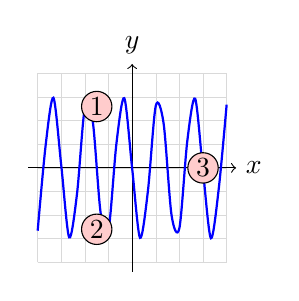
\begin{tikzpicture}[scale=0.6]
\draw[step=0.5,gray!30,very thin] (-2,-2) grid (2,2);
\draw[->] (-2.2,0) -- (2.2,0) node[right] {$x$};
\draw[->] (0,-2.2) -- (0,2.2) node[above] {$y$};
\draw[domain=-2:2,smooth,variable=\x,blue,thick] plot ({\x},{sin(\x*67 r)*1.5});
\foreach \a in {1,...,3} \node[circle,draw,fill=red!20,inner sep=1pt] at ({360/3*\a}:1.5) {\a};
\end{tikzpicture}
\par\medskip
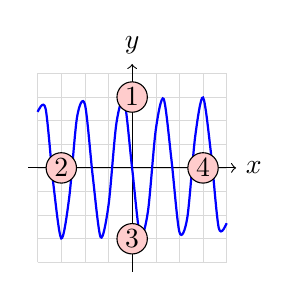
\begin{tikzpicture}[scale=0.6]
\draw[step=0.5,gray!30,very thin] (-2,-2) grid (2,2);
\draw[->] (-2.2,0) -- (2.2,0) node[right] {$x$};
\draw[->] (0,-2.2) -- (0,2.2) node[above] {$y$};
\draw[domain=-2:2,smooth,variable=\x,blue,thick] plot ({\x},{sin(\x*68 r)*1.5});
\foreach \a in {1,...,4} \node[circle,draw,fill=red!20,inner sep=1pt] at ({360/4*\a}:1.5) {\a};
\end{tikzpicture}
\par\medskip
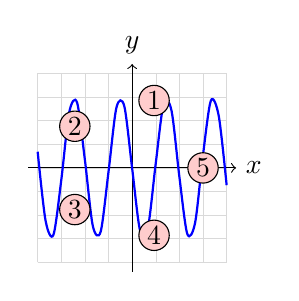
\begin{tikzpicture}[scale=0.6]
\draw[step=0.5,gray!30,very thin] (-2,-2) grid (2,2);
\draw[->] (-2.2,0) -- (2.2,0) node[right] {$x$};
\draw[->] (0,-2.2) -- (0,2.2) node[above] {$y$};
\draw[domain=-2:2,smooth,variable=\x,blue,thick] plot ({\x},{sin(\x*69 r)*1.5});
\foreach \a in {1,...,5} \node[circle,draw,fill=red!20,inner sep=1pt] at ({360/5*\a}:1.5) {\a};
\end{tikzpicture}
\par\medskip
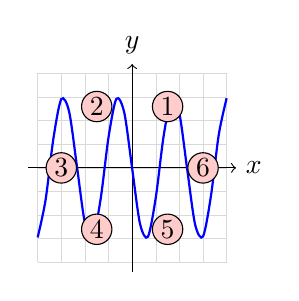
\begin{tikzpicture}[scale=0.6]
\draw[step=0.5,gray!30,very thin] (-2,-2) grid (2,2);
\draw[->] (-2.2,0) -- (2.2,0) node[right] {$x$};
\draw[->] (0,-2.2) -- (0,2.2) node[above] {$y$};
\draw[domain=-2:2,smooth,variable=\x,blue,thick] plot ({\x},{sin(\x*70 r)*1.5});
\foreach \a in {1,...,6} \node[circle,draw,fill=red!20,inner sep=1pt] at ({360/6*\a}:1.5) {\a};
\end{tikzpicture}
\par\medskip
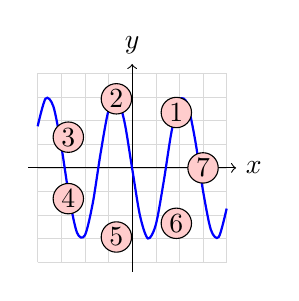
\begin{tikzpicture}[scale=0.6]
\draw[step=0.5,gray!30,very thin] (-2,-2) grid (2,2);
\draw[->] (-2.2,0) -- (2.2,0) node[right] {$x$};
\draw[->] (0,-2.2) -- (0,2.2) node[above] {$y$};
\draw[domain=-2:2,smooth,variable=\x,blue,thick] plot ({\x},{sin(\x*71 r)*1.5});
\foreach \a in {1,...,7} \node[circle,draw,fill=red!20,inner sep=1pt] at ({360/7*\a}:1.5) {\a};
\end{tikzpicture}
\par\medskip
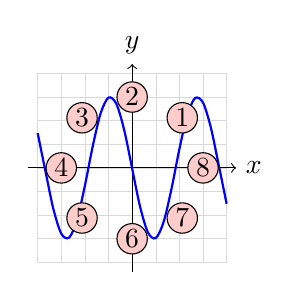
\begin{tikzpicture}[scale=0.6]
\draw[step=0.5,gray!30,very thin] (-2,-2) grid (2,2);
\draw[->] (-2.2,0) -- (2.2,0) node[right] {$x$};
\draw[->] (0,-2.2) -- (0,2.2) node[above] {$y$};
\draw[domain=-2:2,smooth,variable=\x,blue,thick] plot ({\x},{sin(\x*72 r)*1.5});
\foreach \a in {1,...,8} \node[circle,draw,fill=red!20,inner sep=1pt] at ({360/8*\a}:1.5) {\a};
\end{tikzpicture}
\par\medskip
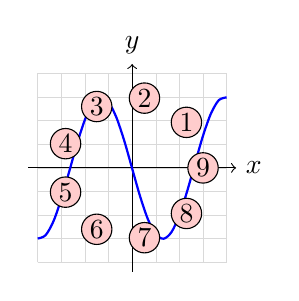
\begin{tikzpicture}[scale=0.6]
\draw[step=0.5,gray!30,very thin] (-2,-2) grid (2,2);
\draw[->] (-2.2,0) -- (2.2,0) node[right] {$x$};
\draw[->] (0,-2.2) -- (0,2.2) node[above] {$y$};
\draw[domain=-2:2,smooth,variable=\x,blue,thick] plot ({\x},{sin(\x*73 r)*1.5});
\foreach \a in {1,...,9} \node[circle,draw,fill=red!20,inner sep=1pt] at ({360/9*\a}:1.5) {\a};
\end{tikzpicture}
\par\medskip
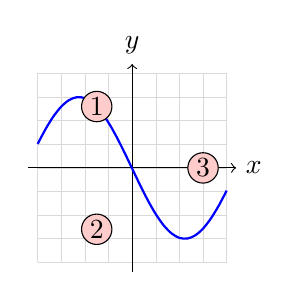
\begin{tikzpicture}[scale=0.6]
\draw[step=0.5,gray!30,very thin] (-2,-2) grid (2,2);
\draw[->] (-2.2,0) -- (2.2,0) node[right] {$x$};
\draw[->] (0,-2.2) -- (0,2.2) node[above] {$y$};
\draw[domain=-2:2,smooth,variable=\x,blue,thick] plot ({\x},{sin(\x*74 r)*1.5});
\foreach \a in {1,...,3} \node[circle,draw,fill=red!20,inner sep=1pt] at ({360/3*\a}:1.5) {\a};
\end{tikzpicture}
\par\medskip
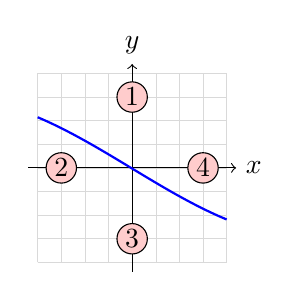
\begin{tikzpicture}[scale=0.6]
\draw[step=0.5,gray!30,very thin] (-2,-2) grid (2,2);
\draw[->] (-2.2,0) -- (2.2,0) node[right] {$x$};
\draw[->] (0,-2.2) -- (0,2.2) node[above] {$y$};
\draw[domain=-2:2,smooth,variable=\x,blue,thick] plot ({\x},{sin(\x*75 r)*1.5});
\foreach \a in {1,...,4} \node[circle,draw,fill=red!20,inner sep=1pt] at ({360/4*\a}:1.5) {\a};
\end{tikzpicture}
\par\medskip
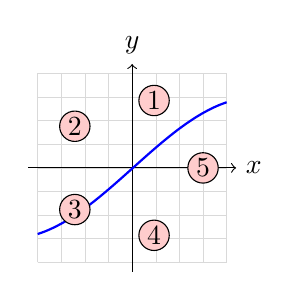
\begin{tikzpicture}[scale=0.6]
\draw[step=0.5,gray!30,very thin] (-2,-2) grid (2,2);
\draw[->] (-2.2,0) -- (2.2,0) node[right] {$x$};
\draw[->] (0,-2.2) -- (0,2.2) node[above] {$y$};
\draw[domain=-2:2,smooth,variable=\x,blue,thick] plot ({\x},{sin(\x*76 r)*1.5});
\foreach \a in {1,...,5} \node[circle,draw,fill=red!20,inner sep=1pt] at ({360/5*\a}:1.5) {\a};
\end{tikzpicture}
\par\medskip
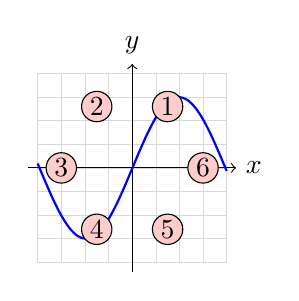
\begin{tikzpicture}[scale=0.6]
\draw[step=0.5,gray!30,very thin] (-2,-2) grid (2,2);
\draw[->] (-2.2,0) -- (2.2,0) node[right] {$x$};
\draw[->] (0,-2.2) -- (0,2.2) node[above] {$y$};
\draw[domain=-2:2,smooth,variable=\x,blue,thick] plot ({\x},{sin(\x*77 r)*1.5});
\foreach \a in {1,...,6} \node[circle,draw,fill=red!20,inner sep=1pt] at ({360/6*\a}:1.5) {\a};
\end{tikzpicture}
\par\medskip
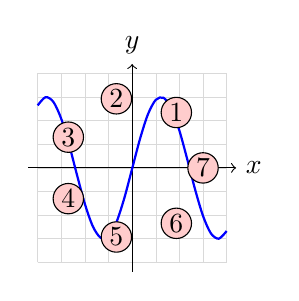
\begin{tikzpicture}[scale=0.6]
\draw[step=0.5,gray!30,very thin] (-2,-2) grid (2,2);
\draw[->] (-2.2,0) -- (2.2,0) node[right] {$x$};
\draw[->] (0,-2.2) -- (0,2.2) node[above] {$y$};
\draw[domain=-2:2,smooth,variable=\x,blue,thick] plot ({\x},{sin(\x*78 r)*1.5});
\foreach \a in {1,...,7} \node[circle,draw,fill=red!20,inner sep=1pt] at ({360/7*\a}:1.5) {\a};
\end{tikzpicture}
\par\medskip
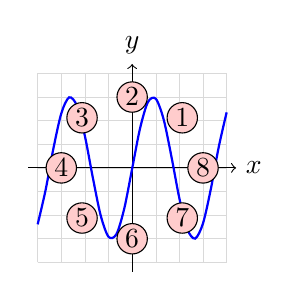
\begin{tikzpicture}[scale=0.6]
\draw[step=0.5,gray!30,very thin] (-2,-2) grid (2,2);
\draw[->] (-2.2,0) -- (2.2,0) node[right] {$x$};
\draw[->] (0,-2.2) -- (0,2.2) node[above] {$y$};
\draw[domain=-2:2,smooth,variable=\x,blue,thick] plot ({\x},{sin(\x*79 r)*1.5});
\foreach \a in {1,...,8} \node[circle,draw,fill=red!20,inner sep=1pt] at ({360/8*\a}:1.5) {\a};
\end{tikzpicture}
\par\medskip
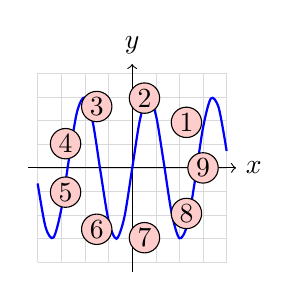
\begin{tikzpicture}[scale=0.6]
\draw[step=0.5,gray!30,very thin] (-2,-2) grid (2,2);
\draw[->] (-2.2,0) -- (2.2,0) node[right] {$x$};
\draw[->] (0,-2.2) -- (0,2.2) node[above] {$y$};
\draw[domain=-2:2,smooth,variable=\x,blue,thick] plot ({\x},{sin(\x*80 r)*1.5});
\foreach \a in {1,...,9} \node[circle,draw,fill=red!20,inner sep=1pt] at ({360/9*\a}:1.5) {\a};
\end{tikzpicture}
\par\medskip
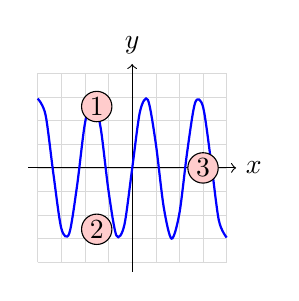
\begin{tikzpicture}[scale=0.6]
\draw[step=0.5,gray!30,very thin] (-2,-2) grid (2,2);
\draw[->] (-2.2,0) -- (2.2,0) node[right] {$x$};
\draw[->] (0,-2.2) -- (0,2.2) node[above] {$y$};
\draw[domain=-2:2,smooth,variable=\x,blue,thick] plot ({\x},{sin(\x*81 r)*1.5});
\foreach \a in {1,...,3} \node[circle,draw,fill=red!20,inner sep=1pt] at ({360/3*\a}:1.5) {\a};
\end{tikzpicture}
\par\medskip
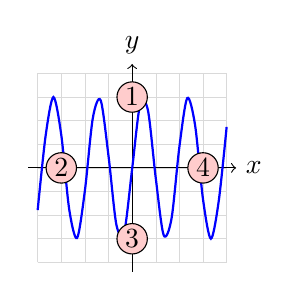
\begin{tikzpicture}[scale=0.6]
\draw[step=0.5,gray!30,very thin] (-2,-2) grid (2,2);
\draw[->] (-2.2,0) -- (2.2,0) node[right] {$x$};
\draw[->] (0,-2.2) -- (0,2.2) node[above] {$y$};
\draw[domain=-2:2,smooth,variable=\x,blue,thick] plot ({\x},{sin(\x*82 r)*1.5});
\foreach \a in {1,...,4} \node[circle,draw,fill=red!20,inner sep=1pt] at ({360/4*\a}:1.5) {\a};
\end{tikzpicture}
\par\medskip
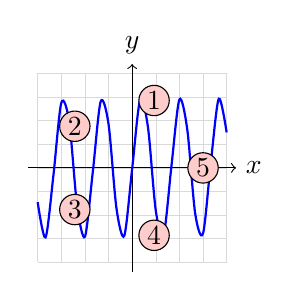
\begin{tikzpicture}[scale=0.6]
\draw[step=0.5,gray!30,very thin] (-2,-2) grid (2,2);
\draw[->] (-2.2,0) -- (2.2,0) node[right] {$x$};
\draw[->] (0,-2.2) -- (0,2.2) node[above] {$y$};
\draw[domain=-2:2,smooth,variable=\x,blue,thick] plot ({\x},{sin(\x*83 r)*1.5});
\foreach \a in {1,...,5} \node[circle,draw,fill=red!20,inner sep=1pt] at ({360/5*\a}:1.5) {\a};
\end{tikzpicture}
\par\medskip
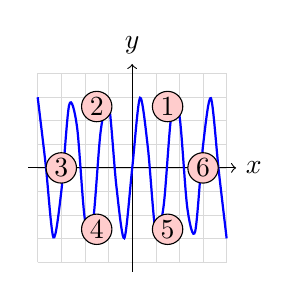
\begin{tikzpicture}[scale=0.6]
\draw[step=0.5,gray!30,very thin] (-2,-2) grid (2,2);
\draw[->] (-2.2,0) -- (2.2,0) node[right] {$x$};
\draw[->] (0,-2.2) -- (0,2.2) node[above] {$y$};
\draw[domain=-2:2,smooth,variable=\x,blue,thick] plot ({\x},{sin(\x*84 r)*1.5});
\foreach \a in {1,...,6} \node[circle,draw,fill=red!20,inner sep=1pt] at ({360/6*\a}:1.5) {\a};
\end{tikzpicture}
\par\medskip
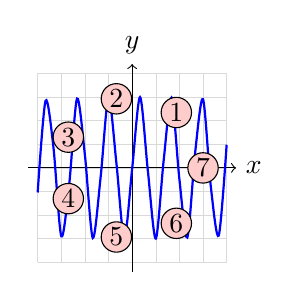
\begin{tikzpicture}[scale=0.6]
\draw[step=0.5,gray!30,very thin] (-2,-2) grid (2,2);
\draw[->] (-2.2,0) -- (2.2,0) node[right] {$x$};
\draw[->] (0,-2.2) -- (0,2.2) node[above] {$y$};
\draw[domain=-2:2,smooth,variable=\x,blue,thick] plot ({\x},{sin(\x*85 r)*1.5});
\foreach \a in {1,...,7} \node[circle,draw,fill=red!20,inner sep=1pt] at ({360/7*\a}:1.5) {\a};
\end{tikzpicture}
\par\medskip
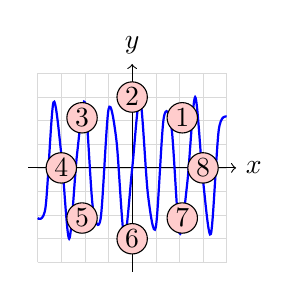
\begin{tikzpicture}[scale=0.6]
\draw[step=0.5,gray!30,very thin] (-2,-2) grid (2,2);
\draw[->] (-2.2,0) -- (2.2,0) node[right] {$x$};
\draw[->] (0,-2.2) -- (0,2.2) node[above] {$y$};
\draw[domain=-2:2,smooth,variable=\x,blue,thick] plot ({\x},{sin(\x*86 r)*1.5});
\foreach \a in {1,...,8} \node[circle,draw,fill=red!20,inner sep=1pt] at ({360/8*\a}:1.5) {\a};
\end{tikzpicture}
\par\medskip
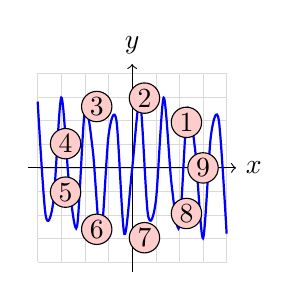
\begin{tikzpicture}[scale=0.6]
\draw[step=0.5,gray!30,very thin] (-2,-2) grid (2,2);
\draw[->] (-2.2,0) -- (2.2,0) node[right] {$x$};
\draw[->] (0,-2.2) -- (0,2.2) node[above] {$y$};
\draw[domain=-2:2,smooth,variable=\x,blue,thick] plot ({\x},{sin(\x*87 r)*1.5});
\foreach \a in {1,...,9} \node[circle,draw,fill=red!20,inner sep=1pt] at ({360/9*\a}:1.5) {\a};
\end{tikzpicture}
\par\medskip
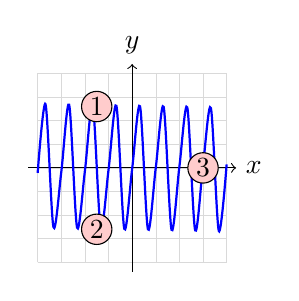
\begin{tikzpicture}[scale=0.6]
\draw[step=0.5,gray!30,very thin] (-2,-2) grid (2,2);
\draw[->] (-2.2,0) -- (2.2,0) node[right] {$x$};
\draw[->] (0,-2.2) -- (0,2.2) node[above] {$y$};
\draw[domain=-2:2,smooth,variable=\x,blue,thick] plot ({\x},{sin(\x*88 r)*1.5});
\foreach \a in {1,...,3} \node[circle,draw,fill=red!20,inner sep=1pt] at ({360/3*\a}:1.5) {\a};
\end{tikzpicture}
\par\medskip
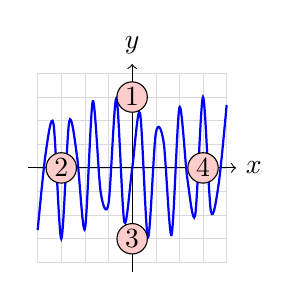
\begin{tikzpicture}[scale=0.6]
\draw[step=0.5,gray!30,very thin] (-2,-2) grid (2,2);
\draw[->] (-2.2,0) -- (2.2,0) node[right] {$x$};
\draw[->] (0,-2.2) -- (0,2.2) node[above] {$y$};
\draw[domain=-2:2,smooth,variable=\x,blue,thick] plot ({\x},{sin(\x*89 r)*1.5});
\foreach \a in {1,...,4} \node[circle,draw,fill=red!20,inner sep=1pt] at ({360/4*\a}:1.5) {\a};
\end{tikzpicture}
\par\medskip
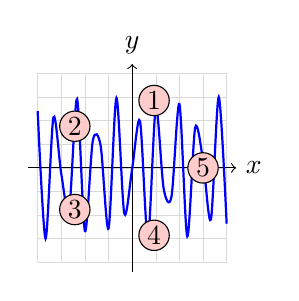
\begin{tikzpicture}[scale=0.6]
\draw[step=0.5,gray!30,very thin] (-2,-2) grid (2,2);
\draw[->] (-2.2,0) -- (2.2,0) node[right] {$x$};
\draw[->] (0,-2.2) -- (0,2.2) node[above] {$y$};
\draw[domain=-2:2,smooth,variable=\x,blue,thick] plot ({\x},{sin(\x*90 r)*1.5});
\foreach \a in {1,...,5} \node[circle,draw,fill=red!20,inner sep=1pt] at ({360/5*\a}:1.5) {\a};
\end{tikzpicture}
\par\medskip
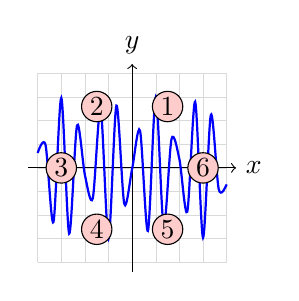
\begin{tikzpicture}[scale=0.6]
\draw[step=0.5,gray!30,very thin] (-2,-2) grid (2,2);
\draw[->] (-2.2,0) -- (2.2,0) node[right] {$x$};
\draw[->] (0,-2.2) -- (0,2.2) node[above] {$y$};
\draw[domain=-2:2,smooth,variable=\x,blue,thick] plot ({\x},{sin(\x*91 r)*1.5});
\foreach \a in {1,...,6} \node[circle,draw,fill=red!20,inner sep=1pt] at ({360/6*\a}:1.5) {\a};
\end{tikzpicture}
\par\medskip
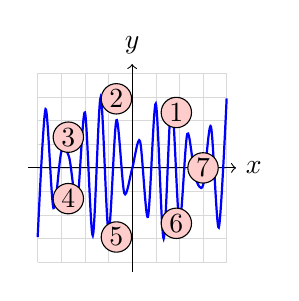
\begin{tikzpicture}[scale=0.6]
\draw[step=0.5,gray!30,very thin] (-2,-2) grid (2,2);
\draw[->] (-2.2,0) -- (2.2,0) node[right] {$x$};
\draw[->] (0,-2.2) -- (0,2.2) node[above] {$y$};
\draw[domain=-2:2,smooth,variable=\x,blue,thick] plot ({\x},{sin(\x*92 r)*1.5});
\foreach \a in {1,...,7} \node[circle,draw,fill=red!20,inner sep=1pt] at ({360/7*\a}:1.5) {\a};
\end{tikzpicture}
\par\medskip
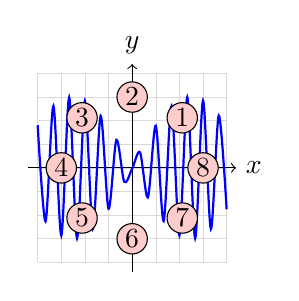
\begin{tikzpicture}[scale=0.6]
\draw[step=0.5,gray!30,very thin] (-2,-2) grid (2,2);
\draw[->] (-2.2,0) -- (2.2,0) node[right] {$x$};
\draw[->] (0,-2.2) -- (0,2.2) node[above] {$y$};
\draw[domain=-2:2,smooth,variable=\x,blue,thick] plot ({\x},{sin(\x*93 r)*1.5});
\foreach \a in {1,...,8} \node[circle,draw,fill=red!20,inner sep=1pt] at ({360/8*\a}:1.5) {\a};
\end{tikzpicture}
\par\medskip
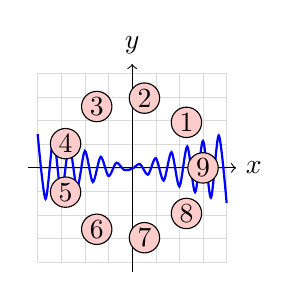
\begin{tikzpicture}[scale=0.6]
\draw[step=0.5,gray!30,very thin] (-2,-2) grid (2,2);
\draw[->] (-2.2,0) -- (2.2,0) node[right] {$x$};
\draw[->] (0,-2.2) -- (0,2.2) node[above] {$y$};
\draw[domain=-2:2,smooth,variable=\x,blue,thick] plot ({\x},{sin(\x*94 r)*1.5});
\foreach \a in {1,...,9} \node[circle,draw,fill=red!20,inner sep=1pt] at ({360/9*\a}:1.5) {\a};
\end{tikzpicture}
\par\medskip
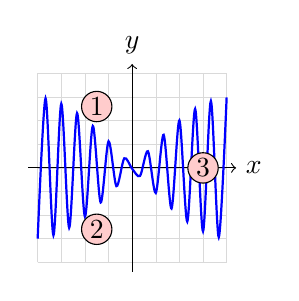
\begin{tikzpicture}[scale=0.6]
\draw[step=0.5,gray!30,very thin] (-2,-2) grid (2,2);
\draw[->] (-2.2,0) -- (2.2,0) node[right] {$x$};
\draw[->] (0,-2.2) -- (0,2.2) node[above] {$y$};
\draw[domain=-2:2,smooth,variable=\x,blue,thick] plot ({\x},{sin(\x*95 r)*1.5});
\foreach \a in {1,...,3} \node[circle,draw,fill=red!20,inner sep=1pt] at ({360/3*\a}:1.5) {\a};
\end{tikzpicture}
\par\medskip
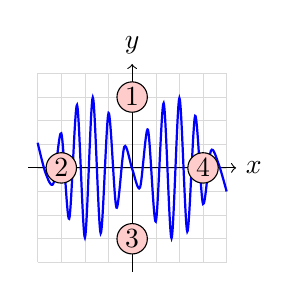
\begin{tikzpicture}[scale=0.6]
\draw[step=0.5,gray!30,very thin] (-2,-2) grid (2,2);
\draw[->] (-2.2,0) -- (2.2,0) node[right] {$x$};
\draw[->] (0,-2.2) -- (0,2.2) node[above] {$y$};
\draw[domain=-2:2,smooth,variable=\x,blue,thick] plot ({\x},{sin(\x*96 r)*1.5});
\foreach \a in {1,...,4} \node[circle,draw,fill=red!20,inner sep=1pt] at ({360/4*\a}:1.5) {\a};
\end{tikzpicture}
\par\medskip
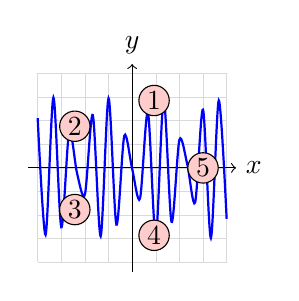
\begin{tikzpicture}[scale=0.6]
\draw[step=0.5,gray!30,very thin] (-2,-2) grid (2,2);
\draw[->] (-2.2,0) -- (2.2,0) node[right] {$x$};
\draw[->] (0,-2.2) -- (0,2.2) node[above] {$y$};
\draw[domain=-2:2,smooth,variable=\x,blue,thick] plot ({\x},{sin(\x*97 r)*1.5});
\foreach \a in {1,...,5} \node[circle,draw,fill=red!20,inner sep=1pt] at ({360/5*\a}:1.5) {\a};
\end{tikzpicture}
\par\medskip
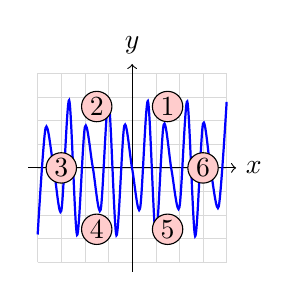
\begin{tikzpicture}[scale=0.6]
\draw[step=0.5,gray!30,very thin] (-2,-2) grid (2,2);
\draw[->] (-2.2,0) -- (2.2,0) node[right] {$x$};
\draw[->] (0,-2.2) -- (0,2.2) node[above] {$y$};
\draw[domain=-2:2,smooth,variable=\x,blue,thick] plot ({\x},{sin(\x*98 r)*1.5});
\foreach \a in {1,...,6} \node[circle,draw,fill=red!20,inner sep=1pt] at ({360/6*\a}:1.5) {\a};
\end{tikzpicture}
\par\medskip
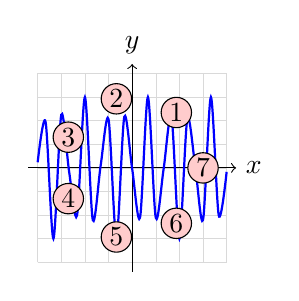
\begin{tikzpicture}[scale=0.6]
\draw[step=0.5,gray!30,very thin] (-2,-2) grid (2,2);
\draw[->] (-2.2,0) -- (2.2,0) node[right] {$x$};
\draw[->] (0,-2.2) -- (0,2.2) node[above] {$y$};
\draw[domain=-2:2,smooth,variable=\x,blue,thick] plot ({\x},{sin(\x*99 r)*1.5});
\foreach \a in {1,...,7} \node[circle,draw,fill=red!20,inner sep=1pt] at ({360/7*\a}:1.5) {\a};
\end{tikzpicture}
\par\medskip
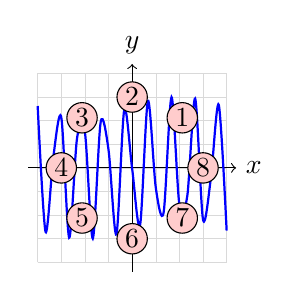
\begin{tikzpicture}[scale=0.6]
\draw[step=0.5,gray!30,very thin] (-2,-2) grid (2,2);
\draw[->] (-2.2,0) -- (2.2,0) node[right] {$x$};
\draw[->] (0,-2.2) -- (0,2.2) node[above] {$y$};
\draw[domain=-2:2,smooth,variable=\x,blue,thick] plot ({\x},{sin(\x*100 r)*1.5});
\foreach \a in {1,...,8} \node[circle,draw,fill=red!20,inner sep=1pt] at ({360/8*\a}:1.5) {\a};
\end{tikzpicture}
\par\medskip
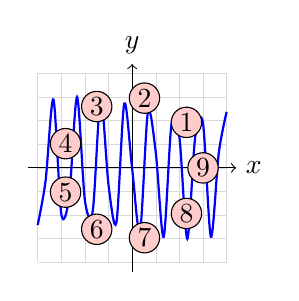
\begin{tikzpicture}[scale=0.6]
\draw[step=0.5,gray!30,very thin] (-2,-2) grid (2,2);
\draw[->] (-2.2,0) -- (2.2,0) node[right] {$x$};
\draw[->] (0,-2.2) -- (0,2.2) node[above] {$y$};
\draw[domain=-2:2,smooth,variable=\x,blue,thick] plot ({\x},{sin(\x*101 r)*1.5});
\foreach \a in {1,...,9} \node[circle,draw,fill=red!20,inner sep=1pt] at ({360/9*\a}:1.5) {\a};
\end{tikzpicture}
\par\medskip
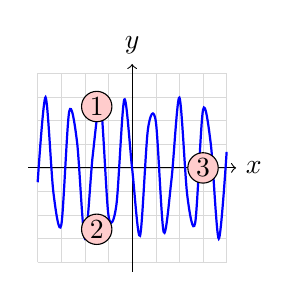
\begin{tikzpicture}[scale=0.6]
\draw[step=0.5,gray!30,very thin] (-2,-2) grid (2,2);
\draw[->] (-2.2,0) -- (2.2,0) node[right] {$x$};
\draw[->] (0,-2.2) -- (0,2.2) node[above] {$y$};
\draw[domain=-2:2,smooth,variable=\x,blue,thick] plot ({\x},{sin(\x*102 r)*1.5});
\foreach \a in {1,...,3} \node[circle,draw,fill=red!20,inner sep=1pt] at ({360/3*\a}:1.5) {\a};
\end{tikzpicture}
\par\medskip
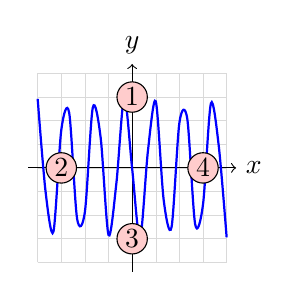
\begin{tikzpicture}[scale=0.6]
\draw[step=0.5,gray!30,very thin] (-2,-2) grid (2,2);
\draw[->] (-2.2,0) -- (2.2,0) node[right] {$x$};
\draw[->] (0,-2.2) -- (0,2.2) node[above] {$y$};
\draw[domain=-2:2,smooth,variable=\x,blue,thick] plot ({\x},{sin(\x*103 r)*1.5});
\foreach \a in {1,...,4} \node[circle,draw,fill=red!20,inner sep=1pt] at ({360/4*\a}:1.5) {\a};
\end{tikzpicture}
\par\medskip
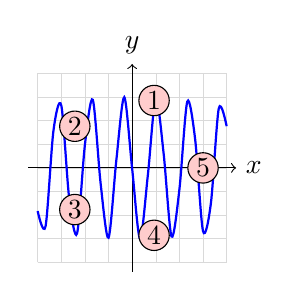
\begin{tikzpicture}[scale=0.6]
\draw[step=0.5,gray!30,very thin] (-2,-2) grid (2,2);
\draw[->] (-2.2,0) -- (2.2,0) node[right] {$x$};
\draw[->] (0,-2.2) -- (0,2.2) node[above] {$y$};
\draw[domain=-2:2,smooth,variable=\x,blue,thick] plot ({\x},{sin(\x*104 r)*1.5});
\foreach \a in {1,...,5} \node[circle,draw,fill=red!20,inner sep=1pt] at ({360/5*\a}:1.5) {\a};
\end{tikzpicture}
\par\medskip
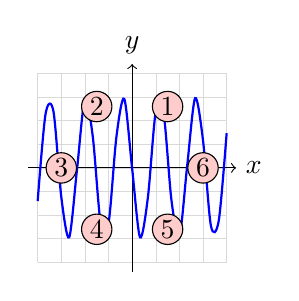
\begin{tikzpicture}[scale=0.6]
\draw[step=0.5,gray!30,very thin] (-2,-2) grid (2,2);
\draw[->] (-2.2,0) -- (2.2,0) node[right] {$x$};
\draw[->] (0,-2.2) -- (0,2.2) node[above] {$y$};
\draw[domain=-2:2,smooth,variable=\x,blue,thick] plot ({\x},{sin(\x*105 r)*1.5});
\foreach \a in {1,...,6} \node[circle,draw,fill=red!20,inner sep=1pt] at ({360/6*\a}:1.5) {\a};
\end{tikzpicture}
\par\medskip
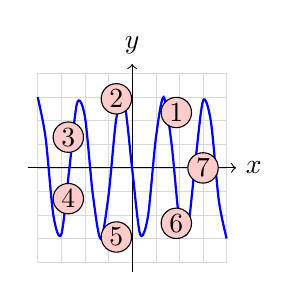
\begin{tikzpicture}[scale=0.6]
\draw[step=0.5,gray!30,very thin] (-2,-2) grid (2,2);
\draw[->] (-2.2,0) -- (2.2,0) node[right] {$x$};
\draw[->] (0,-2.2) -- (0,2.2) node[above] {$y$};
\draw[domain=-2:2,smooth,variable=\x,blue,thick] plot ({\x},{sin(\x*106 r)*1.5});
\foreach \a in {1,...,7} \node[circle,draw,fill=red!20,inner sep=1pt] at ({360/7*\a}:1.5) {\a};
\end{tikzpicture}
\par\medskip
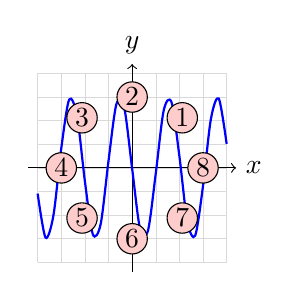
\begin{tikzpicture}[scale=0.6]
\draw[step=0.5,gray!30,very thin] (-2,-2) grid (2,2);
\draw[->] (-2.2,0) -- (2.2,0) node[right] {$x$};
\draw[->] (0,-2.2) -- (0,2.2) node[above] {$y$};
\draw[domain=-2:2,smooth,variable=\x,blue,thick] plot ({\x},{sin(\x*107 r)*1.5});
\foreach \a in {1,...,8} \node[circle,draw,fill=red!20,inner sep=1pt] at ({360/8*\a}:1.5) {\a};
\end{tikzpicture}
\par\medskip
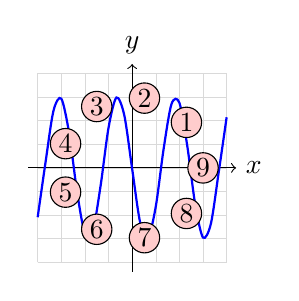
\begin{tikzpicture}[scale=0.6]
\draw[step=0.5,gray!30,very thin] (-2,-2) grid (2,2);
\draw[->] (-2.2,0) -- (2.2,0) node[right] {$x$};
\draw[->] (0,-2.2) -- (0,2.2) node[above] {$y$};
\draw[domain=-2:2,smooth,variable=\x,blue,thick] plot ({\x},{sin(\x*108 r)*1.5});
\foreach \a in {1,...,9} \node[circle,draw,fill=red!20,inner sep=1pt] at ({360/9*\a}:1.5) {\a};
\end{tikzpicture}
\par\medskip
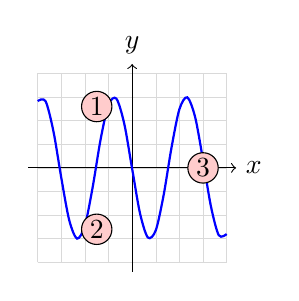
\begin{tikzpicture}[scale=0.6]
\draw[step=0.5,gray!30,very thin] (-2,-2) grid (2,2);
\draw[->] (-2.2,0) -- (2.2,0) node[right] {$x$};
\draw[->] (0,-2.2) -- (0,2.2) node[above] {$y$};
\draw[domain=-2:2,smooth,variable=\x,blue,thick] plot ({\x},{sin(\x*109 r)*1.5});
\foreach \a in {1,...,3} \node[circle,draw,fill=red!20,inner sep=1pt] at ({360/3*\a}:1.5) {\a};
\end{tikzpicture}
\par\medskip
\begin{tikzpicture}[scale=0.6]
\draw[step=0.5,gray!30,very thin] (-2,-2) grid (2,2);
\draw[->] (-2.2,0) -- (2.2,0) node[right] {$x$};
\draw[->] (0,-2.2) -- (0,2.2) node[above] {$y$};
\draw[domain=-2:2,smooth,variable=\x,blue,thick] plot ({\x},{sin(\x*110 r)*1.5});
\foreach \a in {1,...,4} \node[circle,draw,fill=red!20,inner sep=1pt] at ({360/4*\a}:1.5) {\a};
\end{tikzpicture}
\par\medskip
\begin{tikzpicture}[scale=0.6]
\draw[step=0.5,gray!30,very thin] (-2,-2) grid (2,2);
\draw[->] (-2.2,0) -- (2.2,0) node[right] {$x$};
\draw[->] (0,-2.2) -- (0,2.2) node[above] {$y$};
\draw[domain=-2:2,smooth,variable=\x,blue,thick] plot ({\x},{sin(\x*111 r)*1.5});
\foreach \a in {1,...,5} \node[circle,draw,fill=red!20,inner sep=1pt] at ({360/5*\a}:1.5) {\a};
\end{tikzpicture}
\par\medskip
\begin{tikzpicture}[scale=0.6]
\draw[step=0.5,gray!30,very thin] (-2,-2) grid (2,2);
\draw[->] (-2.2,0) -- (2.2,0) node[right] {$x$};
\draw[->] (0,-2.2) -- (0,2.2) node[above] {$y$};
\draw[domain=-2:2,smooth,variable=\x,blue,thick] plot ({\x},{sin(\x*112 r)*1.5});
\foreach \a in {1,...,6} \node[circle,draw,fill=red!20,inner sep=1pt] at ({360/6*\a}:1.5) {\a};
\end{tikzpicture}
\par\medskip
\begin{tikzpicture}[scale=0.6]
\draw[step=0.5,gray!30,very thin] (-2,-2) grid (2,2);
\draw[->] (-2.2,0) -- (2.2,0) node[right] {$x$};
\draw[->] (0,-2.2) -- (0,2.2) node[above] {$y$};
\draw[domain=-2:2,smooth,variable=\x,blue,thick] plot ({\x},{sin(\x*113 r)*1.5});
\foreach \a in {1,...,7} \node[circle,draw,fill=red!20,inner sep=1pt] at ({360/7*\a}:1.5) {\a};
\end{tikzpicture}
\par\medskip
\begin{tikzpicture}[scale=0.6]
\draw[step=0.5,gray!30,very thin] (-2,-2) grid (2,2);
\draw[->] (-2.2,0) -- (2.2,0) node[right] {$x$};
\draw[->] (0,-2.2) -- (0,2.2) node[above] {$y$};
\draw[domain=-2:2,smooth,variable=\x,blue,thick] plot ({\x},{sin(\x*114 r)*1.5});
\foreach \a in {1,...,8} \node[circle,draw,fill=red!20,inner sep=1pt] at ({360/8*\a}:1.5) {\a};
\end{tikzpicture}
\par\medskip
\begin{tikzpicture}[scale=0.6]
\draw[step=0.5,gray!30,very thin] (-2,-2) grid (2,2);
\draw[->] (-2.2,0) -- (2.2,0) node[right] {$x$};
\draw[->] (0,-2.2) -- (0,2.2) node[above] {$y$};
\draw[domain=-2:2,smooth,variable=\x,blue,thick] plot ({\x},{sin(\x*115 r)*1.5});
\foreach \a in {1,...,9} \node[circle,draw,fill=red!20,inner sep=1pt] at ({360/9*\a}:1.5) {\a};
\end{tikzpicture}
\par\medskip
\begin{tikzpicture}[scale=0.6]
\draw[step=0.5,gray!30,very thin] (-2,-2) grid (2,2);
\draw[->] (-2.2,0) -- (2.2,0) node[right] {$x$};
\draw[->] (0,-2.2) -- (0,2.2) node[above] {$y$};
\draw[domain=-2:2,smooth,variable=\x,blue,thick] plot ({\x},{sin(\x*116 r)*1.5});
\foreach \a in {1,...,3} \node[circle,draw,fill=red!20,inner sep=1pt] at ({360/3*\a}:1.5) {\a};
\end{tikzpicture}
\par\medskip
\begin{tikzpicture}[scale=0.6]
\draw[step=0.5,gray!30,very thin] (-2,-2) grid (2,2);
\draw[->] (-2.2,0) -- (2.2,0) node[right] {$x$};
\draw[->] (0,-2.2) -- (0,2.2) node[above] {$y$};
\draw[domain=-2:2,smooth,variable=\x,blue,thick] plot ({\x},{sin(\x*117 r)*1.5});
\foreach \a in {1,...,4} \node[circle,draw,fill=red!20,inner sep=1pt] at ({360/4*\a}:1.5) {\a};
\end{tikzpicture}
\par\medskip
\begin{tikzpicture}[scale=0.6]
\draw[step=0.5,gray!30,very thin] (-2,-2) grid (2,2);
\draw[->] (-2.2,0) -- (2.2,0) node[right] {$x$};
\draw[->] (0,-2.2) -- (0,2.2) node[above] {$y$};
\draw[domain=-2:2,smooth,variable=\x,blue,thick] plot ({\x},{sin(\x*118 r)*1.5});
\foreach \a in {1,...,5} \node[circle,draw,fill=red!20,inner sep=1pt] at ({360/5*\a}:1.5) {\a};
\end{tikzpicture}
\par\medskip
\begin{tikzpicture}[scale=0.6]
\draw[step=0.5,gray!30,very thin] (-2,-2) grid (2,2);
\draw[->] (-2.2,0) -- (2.2,0) node[right] {$x$};
\draw[->] (0,-2.2) -- (0,2.2) node[above] {$y$};
\draw[domain=-2:2,smooth,variable=\x,blue,thick] plot ({\x},{sin(\x*119 r)*1.5});
\foreach \a in {1,...,6} \node[circle,draw,fill=red!20,inner sep=1pt] at ({360/6*\a}:1.5) {\a};
\end{tikzpicture}
\end{document}
